% Created by tikzDevice version 0.12 on 2019-02-08 11:01:07
% !TEX encoding = UTF-8 Unicode
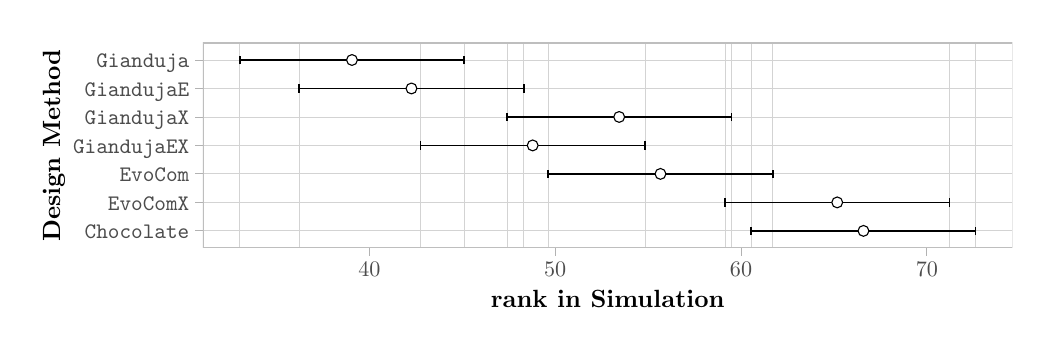
\begin{tikzpicture}[x=1pt,y=1pt]
\definecolor{fillColor}{RGB}{255,255,255}
\path[use as bounding box,fill=fillColor,fill opacity=0.00] (0,0) rectangle (361.35,108.41);
\begin{scope}
\path[clip] (  0.00,  0.00) rectangle (361.35,108.40);
\definecolor{drawColor}{RGB}{255,255,255}
\definecolor{fillColor}{RGB}{255,255,255}

\path[draw=drawColor,line width= 0.6pt,line join=round,line cap=round,fill=fillColor] (  0.00,  0.00) rectangle (361.35,108.40);
\end{scope}
\begin{scope}
\path[clip] ( 63.34, 28.81) rectangle (355.85,102.90);
\definecolor{fillColor}{RGB}{255,255,255}

\path[fill=fillColor] ( 63.34, 28.81) rectangle (355.85,102.90);
\definecolor{drawColor}{RGB}{211,211,211}

\path[draw=drawColor,line width= 0.3pt,line join=round] ( 63.34, 55.57) --
	(355.85, 55.57);

\path[draw=drawColor,line width= 0.3pt,line join=round] ( 63.34, 45.27) --
	(355.85, 45.27);

\path[draw=drawColor,line width= 0.3pt,line join=round] ( 63.34, 96.73) --
	(355.85, 96.73);

\path[draw=drawColor,line width= 0.3pt,line join=round] ( 63.34, 86.44) --
	(355.85, 86.44);

\path[draw=drawColor,line width= 0.3pt,line join=round] ( 63.34, 76.15) --
	(355.85, 76.15);

\path[draw=drawColor,line width= 0.3pt,line join=round] ( 63.34, 65.86) --
	(355.85, 65.86);

\path[draw=drawColor,line width= 0.3pt,line join=round] ( 63.34, 34.98) --
	(355.85, 34.98);

\path[draw=drawColor,line width= 0.2pt,line join=round] (342.55, 28.81) -- (342.55,102.90);

\path[draw=drawColor,line width= 0.2pt,line join=round] (269.21, 28.81) -- (269.21,102.90);

\path[draw=drawColor,line width= 0.2pt,line join=round] (333.08, 28.81) -- (333.08,102.90);

\path[draw=drawColor,line width= 0.2pt,line join=round] (157.74, 28.81) -- (157.74,102.90);

\path[draw=drawColor,line width= 0.2pt,line join=round] (179.23, 28.81) -- (179.23,102.90);

\path[draw=drawColor,line width= 0.2pt,line join=round] (223.02, 28.81) -- (223.02,102.90);

\path[draw=drawColor,line width= 0.2pt,line join=round] (254.29, 28.81) -- (254.29,102.90);

\path[draw=drawColor,line width= 0.2pt,line join=round] (261.46, 28.81) -- (261.46,102.90);

\path[draw=drawColor,line width= 0.2pt,line join=round] (188.11, 28.81) -- (188.11,102.90);

\path[draw=drawColor,line width= 0.2pt,line join=round] (251.98, 28.81) -- (251.98,102.90);

\path[draw=drawColor,line width= 0.2pt,line join=round] ( 76.64, 28.81) -- ( 76.64,102.90);

\path[draw=drawColor,line width= 0.2pt,line join=round] ( 98.13, 28.81) -- ( 98.13,102.90);

\path[draw=drawColor,line width= 0.2pt,line join=round] (141.93, 28.81) -- (141.93,102.90);

\path[draw=drawColor,line width= 0.2pt,line join=round] (173.19, 28.81) -- (173.19,102.90);
\definecolor{drawColor}{RGB}{0,0,0}

\path[draw=drawColor,line width= 0.6pt,line join=round] (342.55, 33.44) --
	(342.55, 36.53);

\path[draw=drawColor,line width= 0.6pt,line join=round] (342.55, 34.98) --
	(261.46, 34.98);

\path[draw=drawColor,line width= 0.6pt,line join=round] (261.46, 33.44) --
	(261.46, 36.53);

\path[draw=drawColor,line width= 0.6pt,line join=round] (269.21, 54.02) --
	(269.21, 57.11);

\path[draw=drawColor,line width= 0.6pt,line join=round] (269.21, 55.57) --
	(188.11, 55.57);

\path[draw=drawColor,line width= 0.6pt,line join=round] (188.11, 54.02) --
	(188.11, 57.11);

\path[draw=drawColor,line width= 0.6pt,line join=round] (333.08, 43.73) --
	(333.08, 46.82);

\path[draw=drawColor,line width= 0.6pt,line join=round] (333.08, 45.27) --
	(251.98, 45.27);

\path[draw=drawColor,line width= 0.6pt,line join=round] (251.98, 43.73) --
	(251.98, 46.82);

\path[draw=drawColor,line width= 0.6pt,line join=round] (157.74, 95.19) --
	(157.74, 98.27);

\path[draw=drawColor,line width= 0.6pt,line join=round] (157.74, 96.73) --
	( 76.64, 96.73);

\path[draw=drawColor,line width= 0.6pt,line join=round] ( 76.64, 95.19) --
	( 76.64, 98.27);

\path[draw=drawColor,line width= 0.6pt,line join=round] (179.23, 84.90) --
	(179.23, 87.98);

\path[draw=drawColor,line width= 0.6pt,line join=round] (179.23, 86.44) --
	( 98.13, 86.44);

\path[draw=drawColor,line width= 0.6pt,line join=round] ( 98.13, 84.90) --
	( 98.13, 87.98);

\path[draw=drawColor,line width= 0.6pt,line join=round] (223.02, 64.31) --
	(223.02, 67.40);

\path[draw=drawColor,line width= 0.6pt,line join=round] (223.02, 65.86) --
	(141.93, 65.86);

\path[draw=drawColor,line width= 0.6pt,line join=round] (141.93, 64.31) --
	(141.93, 67.40);

\path[draw=drawColor,line width= 0.6pt,line join=round] (254.29, 74.60) --
	(254.29, 77.69);

\path[draw=drawColor,line width= 0.6pt,line join=round] (254.29, 76.15) --
	(173.19, 76.15);

\path[draw=drawColor,line width= 0.6pt,line join=round] (173.19, 74.60) --
	(173.19, 77.69);

\path[draw=drawColor,line width= 0.4pt,line join=round,line cap=round,fill=fillColor] (302.01, 34.98) circle (  1.96);

\path[draw=drawColor,line width= 0.4pt,line join=round,line cap=round,fill=fillColor] (228.66, 55.57) circle (  1.96);

\path[draw=drawColor,line width= 0.4pt,line join=round,line cap=round,fill=fillColor] (292.53, 45.27) circle (  1.96);

\path[draw=drawColor,line width= 0.4pt,line join=round,line cap=round,fill=fillColor] (117.19, 96.73) circle (  1.96);

\path[draw=drawColor,line width= 0.4pt,line join=round,line cap=round,fill=fillColor] (138.68, 86.44) circle (  1.96);

\path[draw=drawColor,line width= 0.4pt,line join=round,line cap=round,fill=fillColor] (182.48, 65.86) circle (  1.96);

\path[draw=drawColor,line width= 0.4pt,line join=round,line cap=round,fill=fillColor] (213.74, 76.15) circle (  1.96);
\definecolor{drawColor}{RGB}{190,190,190}

\path[draw=drawColor,line width= 0.6pt,line join=round,line cap=round] ( 63.34, 28.81) rectangle (355.85,102.90);
\end{scope}
\begin{scope}
\path[clip] (  0.00,  0.00) rectangle (361.35,108.41);
\definecolor{drawColor}{gray}{0.30}

\node[text=drawColor,anchor=base east,inner sep=0pt, outer sep=0pt, scale=  0.80] at ( 58.39, 52.81) {\texttt{EvoCom}};

\node[text=drawColor,anchor=base east,inner sep=0pt, outer sep=0pt, scale=  0.80] at ( 58.39, 42.52) {\texttt{EvoComX}};

\node[text=drawColor,anchor=base east,inner sep=0pt, outer sep=0pt, scale=  0.80] at ( 58.39, 93.98) {\texttt{Gianduja}};

\node[text=drawColor,anchor=base east,inner sep=0pt, outer sep=0pt, scale=  0.80] at ( 58.39, 83.68) {\texttt{GiandujaE}};

\node[text=drawColor,anchor=base east,inner sep=0pt, outer sep=0pt, scale=  0.80] at ( 58.39, 73.39) {\texttt{GiandujaX}};

\node[text=drawColor,anchor=base east,inner sep=0pt, outer sep=0pt, scale=  0.80] at ( 58.39, 63.10) {\texttt{GiandujaEX}};

\node[text=drawColor,anchor=base east,inner sep=0pt, outer sep=0pt, scale=  0.80] at ( 58.39, 32.23) {\texttt{Chocolate}};
\end{scope}
\begin{scope}
\path[clip] (  0.00,  0.00) rectangle (361.35,108.41);
\definecolor{drawColor}{gray}{0.70}

\path[draw=drawColor,line width= 0.3pt,line join=round] ( 60.59, 55.57) --
	( 63.34, 55.57);

\path[draw=drawColor,line width= 0.3pt,line join=round] ( 60.59, 45.27) --
	( 63.34, 45.27);

\path[draw=drawColor,line width= 0.3pt,line join=round] ( 60.59, 96.73) --
	( 63.34, 96.73);

\path[draw=drawColor,line width= 0.3pt,line join=round] ( 60.59, 86.44) --
	( 63.34, 86.44);

\path[draw=drawColor,line width= 0.3pt,line join=round] ( 60.59, 76.15) --
	( 63.34, 76.15);

\path[draw=drawColor,line width= 0.3pt,line join=round] ( 60.59, 65.86) --
	( 63.34, 65.86);

\path[draw=drawColor,line width= 0.3pt,line join=round] ( 60.59, 34.98) --
	( 63.34, 34.98);
\end{scope}
\begin{scope}
\path[clip] (  0.00,  0.00) rectangle (361.35,108.41);
\definecolor{drawColor}{gray}{0.70}

\path[draw=drawColor,line width= 0.3pt,line join=round] (123.46, 26.06) --
	(123.46, 28.81);

\path[draw=drawColor,line width= 0.3pt,line join=round] (190.61, 26.06) --
	(190.61, 28.81);

\path[draw=drawColor,line width= 0.3pt,line join=round] (257.76, 26.06) --
	(257.76, 28.81);

\path[draw=drawColor,line width= 0.3pt,line join=round] (324.91, 26.06) --
	(324.91, 28.81);
\end{scope}
\begin{scope}
\path[clip] (  0.00,  0.00) rectangle (361.35,108.41);
\definecolor{drawColor}{gray}{0.30}

\node[text=drawColor,anchor=base,inner sep=0pt, outer sep=0pt, scale=  0.80] at (123.46, 18.35) {40};

\node[text=drawColor,anchor=base,inner sep=0pt, outer sep=0pt, scale=  0.80] at (190.61, 18.35) {50};

\node[text=drawColor,anchor=base,inner sep=0pt, outer sep=0pt, scale=  0.80] at (257.76, 18.35) {60};

\node[text=drawColor,anchor=base,inner sep=0pt, outer sep=0pt, scale=  0.80] at (324.91, 18.35) {70};
\end{scope}
\begin{scope}
\path[clip] (  0.00,  0.00) rectangle (361.35,108.41);
\definecolor{drawColor}{RGB}{0,0,0}

\node[text=drawColor,anchor=base,inner sep=0pt, outer sep=0pt, scale=  0.90] at (209.60,  7.44) {\bfseries rank in Simulation};
\end{scope}
\begin{scope}
\path[clip] (  0.00,  0.00) rectangle (361.35,108.41);
\definecolor{drawColor}{RGB}{0,0,0}

\node[text=drawColor,rotate= 90.00,anchor=base,inner sep=0pt, outer sep=0pt, scale=  0.90] at ( 11.71, 65.86) {\bfseries Design Method};
\end{scope}
\end{tikzpicture}
